\documentclass[journal]{IEEEtran}


\usepackage[utf8]{inputenc}
\usepackage{graphicx}
\usepackage{amsmath}
\usepackage{amsthm}
\usepackage{amssymb}
\usepackage{hyperref}
\usepackage{subfig}
\usepackage{multirow}
\usepackage[section]{placeins}

\usepackage{tabularx,booktabs}
\newcolumntype{C}{>{\centering\arraybackslash}X} % centered version of "X" type
\setlength{\extrarowheight}{1pt}
\usepackage{lipsum}
\usepackage[table]{xcolor}

\renewcommand\thesection{\arabic{section}}


% correct bad hyphenation here
\hyphenation{op-tical net-works semi-conduc-tor}


\begin{document}
\title{Vehicle Driving Assistant}
\author{Akanksha~Dwivedi,
        Anoop~Toffy,
        Athul~Suresh,
        and~Tarini~Chandrashekhar,~\IEEEmembership{International Institute of Information Technology, Bangalore}}% <-this % stops a space




% The paper headers
\markboth{Project Report, \today}%
{Shell \MakeLowercase{\textit{et al.}}: Bare Demo of IEEEtran.cls for IEEE Journals}

\IEEEspecialpapernotice{(Draft Paper)}

% make the title area
\maketitle

% As a general rule, do not put math, special symbols or citations
% in the abstract or keywords.
\begin{abstract}
Autonomous vehicles has been a common term in our day to day life with
car manufacturers like Tesla shipping cars that are SAE Level 3. While
these vehicles include a slew of features such as parking assistance and cruise
control, they’ve mostly been tailored to foreign roads. Potholes, and the
abundance of them, is something that is unique to our Indian roads. We
believe that successful detection of potholes from visual images can be applied
in a variety of scenarios. Moreover, the sheer variety in the color, shape and
size of potholes makes this problem an apt candidate to be solved using
modern machine learning and image processing techniques.
\end{abstract}

% Note that keywords are not normally used for peerreview papers.
\begin{IEEEkeywords}
Image processing, Machine Learning, Pot hole detection, Clustering
\end{IEEEkeywords}

\IEEEpeerreviewmaketitle



\section{Introduction}
The project aims to provide a comprehensive set of assistance features to aid the driver (or autonomous vehicle) to drive safely. This could includes a number of indicators about the environment, the major cue being visualisation and detection of potholes in the road ahead. 

"A pothole \cite{pothole} is a structural failure in a road surface, caused by failure primarily in asphalt pavement due to the presence of water in the underlying soil structure and the presence of traffic passing over the affected area". An example of a road with pothole is shown in Figure 1.

\begin{figure}[!h]
\begin{center}
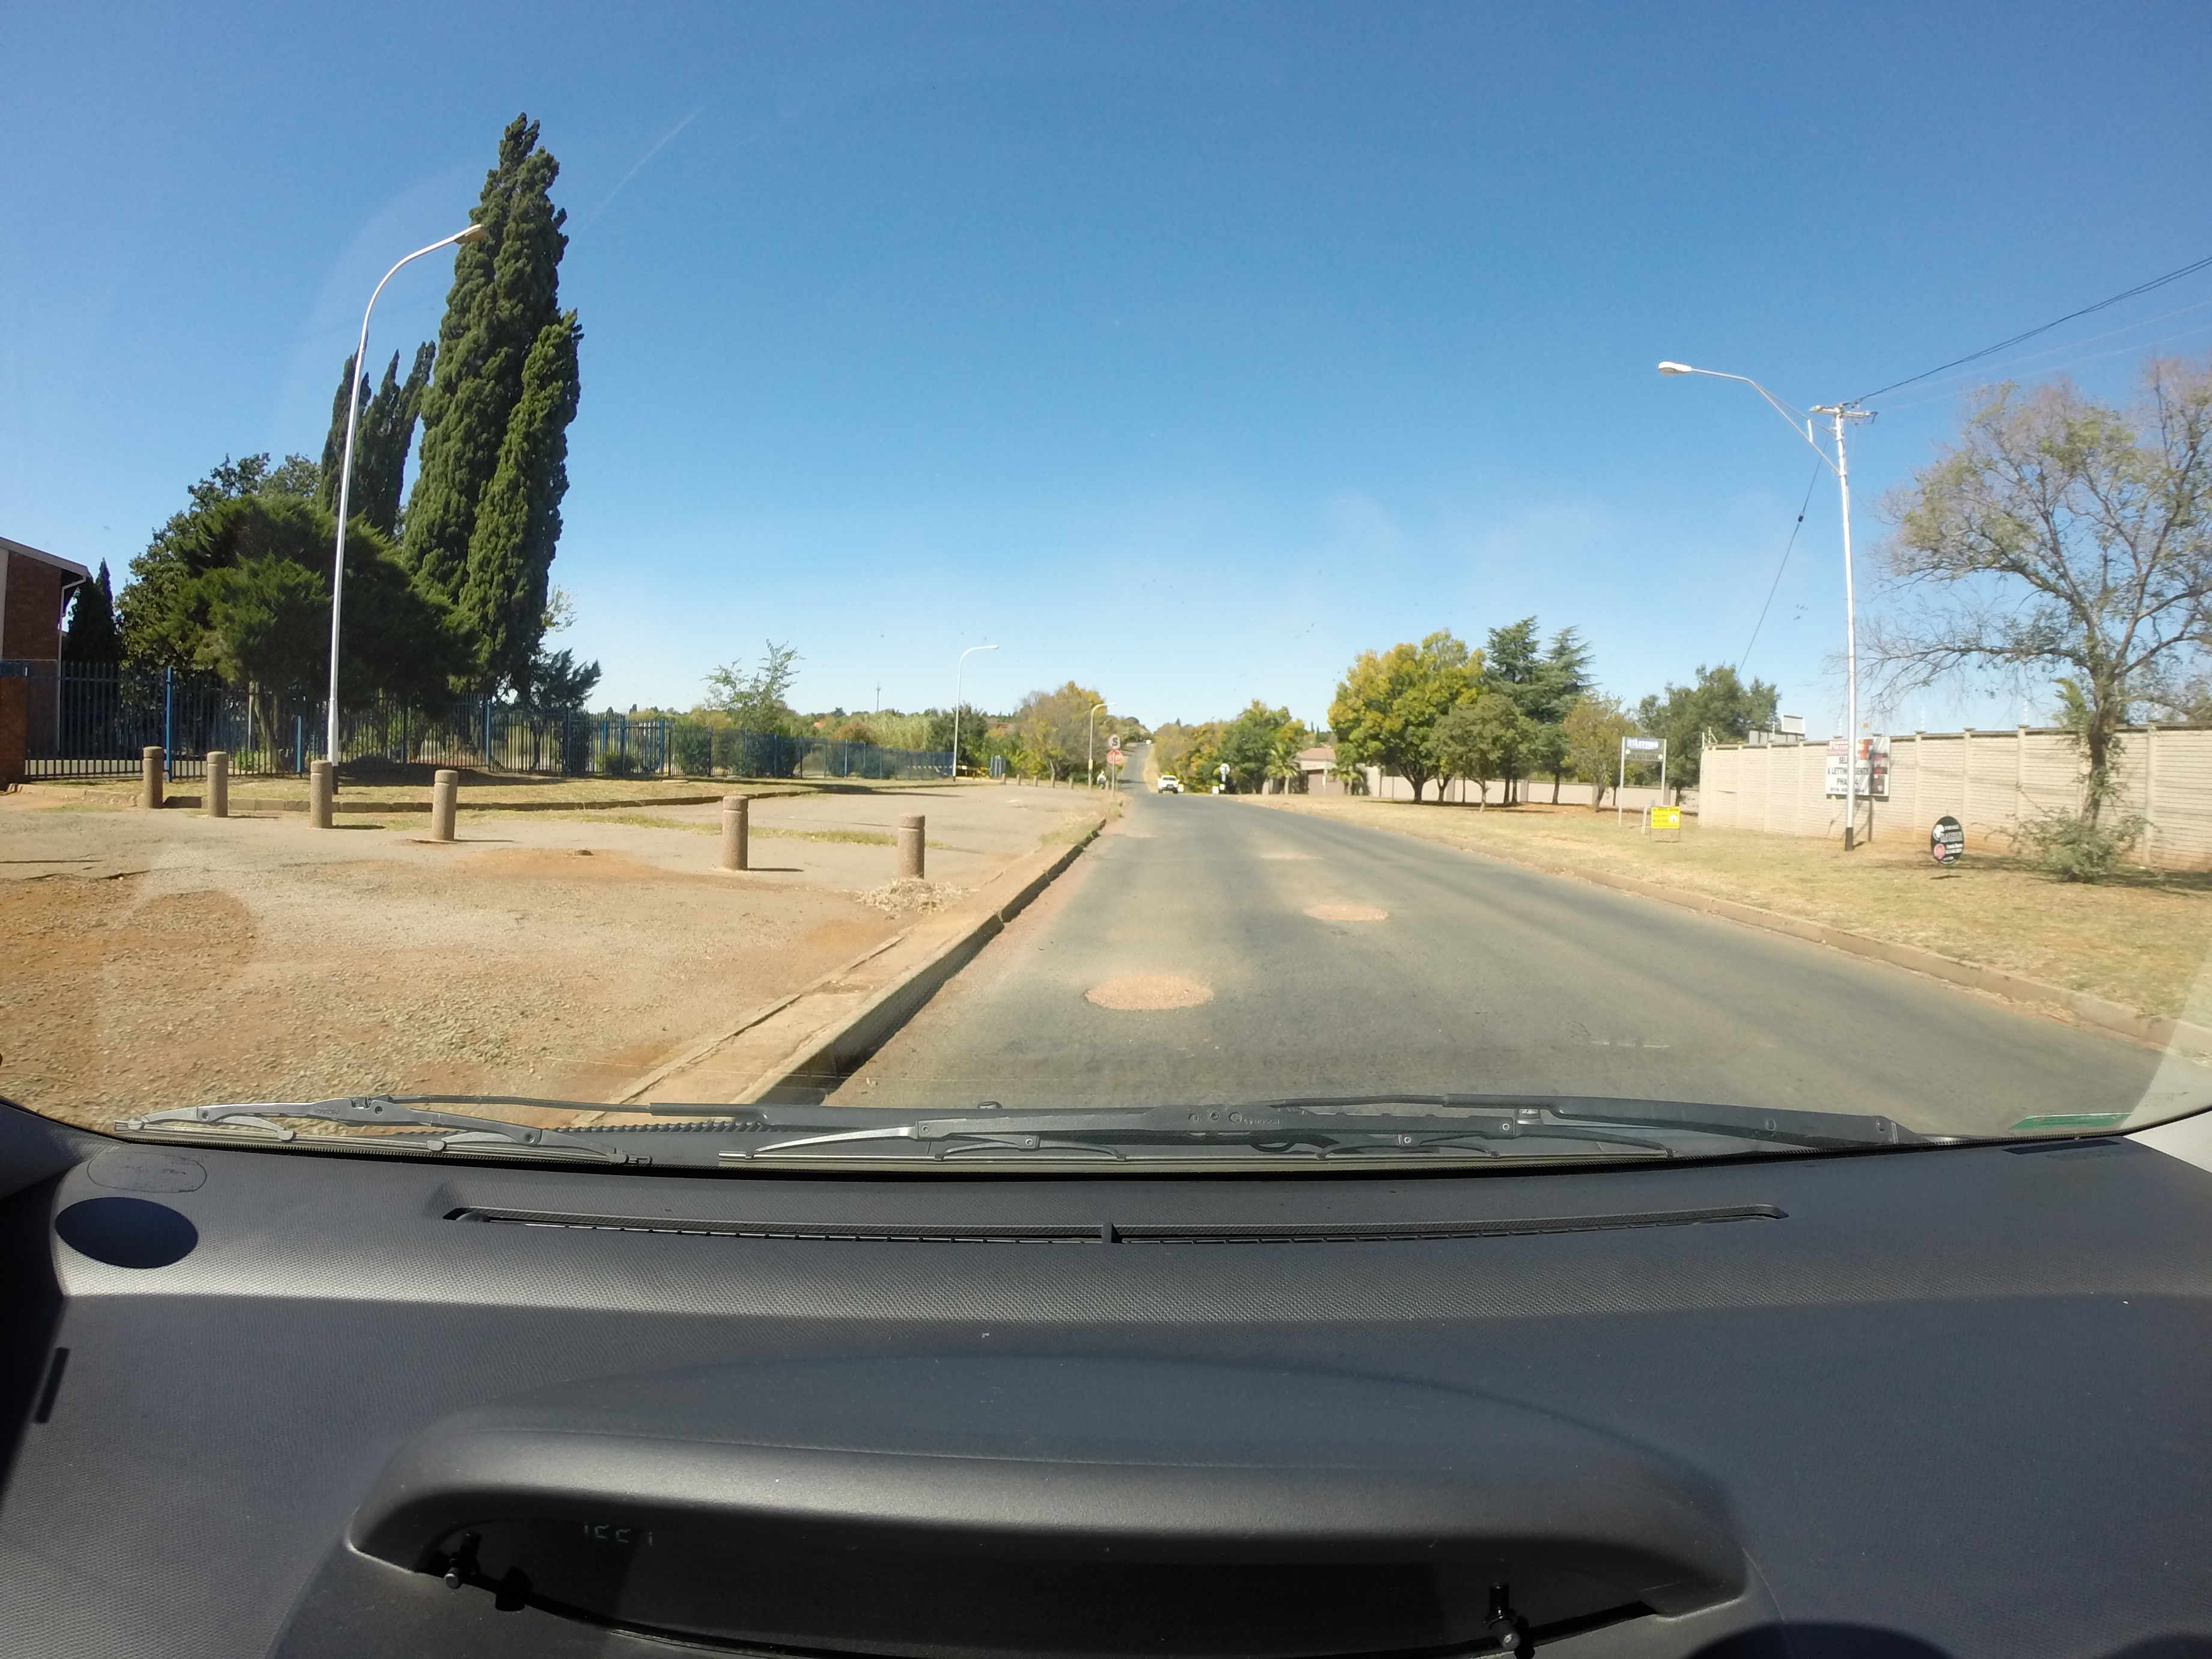
\includegraphics[scale=0.065]{Images/pothole_example.JPG}
\end{center}
\caption{Pothole example}
\end{figure}

The remainder of the paper is structured as follows. We present a brief history of the related work done so far in the field of pothole detection and visualisation in Section 2. Section 3 discusses about the experimental set up we used in this work.In the subsequent section we describes the methodology that we follow in the following section 4. It includes road extraction part and blob detection part. Then the result that we obtained are given briefly in section 5. Finally section 6 concludes the paper. Section 7 gives a light to the future enhancements that could be done.


\section{Related Work}
In Nienaber et al (2015) \cite{paperone}, a system using basic image processing techniques in a constrained environment without relying on any machine learning techniques is used for pothole detection. It presents a good preliminary method for detecting potholes using a single camera within an range of 2 - 20m from a vehicle moving at a speed of not more than 60km/hr. The method separates a rectangular area of interest just above the hood of the vehicle which contains road surface, assuming that driver maintains a safe distance from the front vehicle. The rectangular area of interest is separated by connecting the various farthest region of interest using convex hull algorithm.

\vspace*{.5cm}

The work presented by Ajit Danti et al (2012) \cite{papertwo}, presents a comprehensive approach to address the acute problems of Indian roads such as faded lanes, irregular potholes, improper and invisible road signs. Instead of using image processing techniques for pothole detection as done by Nienaber et al (2015), Ajith Danti et al (2012) uses K-Means clustering based algorithm to detect potholes. By addressing the acute problems above mentioned in the paper it makes automated driving safer and easier in Indian roads. 

\section{Proposed Work}
In this paper we use both image processing techniques as well as machine learning to study the presence and occurrence of potholes. At first we used a Digital camera mounted on the window of a slow moving vehicle (40km/hr) to capture the potholes images. The images are captured at high resolution so that the analysis of the potholes will be easier. This paper propose a way to visualize the potholes as well as identify whether or not the road has a pothole in it. The visualisation approach is similar to how humans perceive the pothole images in the brain. The pothole identification approach will help to signal the driver of a vehicle to take preventive actions upon pothole infected lanes. 

\vspace{0.5cm}

The subsequent subsection describes the approaches we took for visualising the potholes. We used contour detection after applying morphological transformation as a method I and then we used contour detection after extracting the road area by using convex hull algorithm in method II. The methods are described in detail below.

\subsection{Using morphological transformation}

Morphological transformations are some simple operations based on the image shape. It is normally performed on binary images. Two basic morphological operators are Erosion and Dilation. Using which the image is analysed to visualise the pothole present in the region.


\subsection{Using contours and convex hull}

For visualising the pothole we first extract a region of the interest from the given image which will contain the road area. This is done by first selecting the largest contour on the images ROI and then drawing convex hull using convex hull algorithm. Since extracting the road area will help to narrow down the area of interest. This way we will be able to prevent the irrelevant informations from the analysis like foliage, vehicle hood, other vehicles on the road etc. We then apply image processing techniques like contour detection, blob detection and edge detection to draw a bounding box over the area of the road which contains the potholes.

\subsection{Using Machine Learning Methods}
For machine learning technique we used annotated dataset \cite{dataset} for training various classifiers and then try various machine learning algorithms to figure out the presence of a pothole in the frame given.

\section{Methodology}

In this section we briefly familiarize the methodology that we used for the visualisation and detection of potholes in detail. The subsequent section first discusses about the image processing techniques that are helpful for pothole visualisation followed by feature extraction and machine learning learning techniques  used in the study.

\subsection{Pothole Visualisation Techniques}

\subsubsection{Morphological Transformation Method}
We used erosion to detect contours around potholes in the images. Gaussian Blur and thresholding were applied on the input frames to remove the noise signals from the image. The results of Image Gradients: Laplacian, Sobel X, Sobel Y were compared, after applying them on the blurred image. Among all, Sobel Y, performed the best. Then, erosion was applied to this output frame, with the medium sized kernel, to narrow down the search for potholes in the frames. Contours were being detected in the final frame. This technique worked on the Google Images dataset with partial noise being detected but detected too much noise in our dataset along with a fraction of potholes.

\begin{figure}[!htb]
\begin{center}
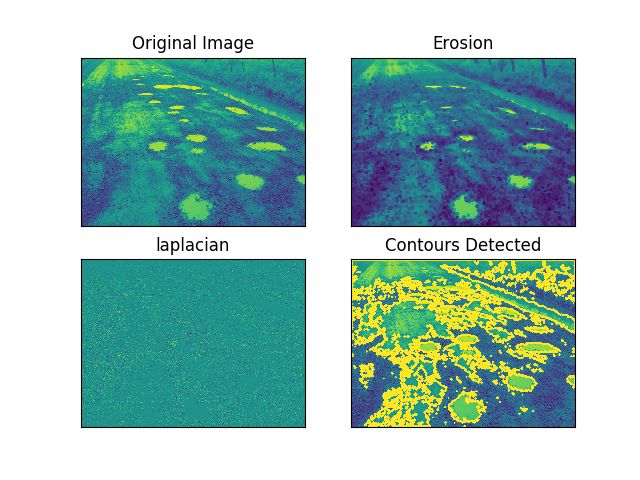
\includegraphics[scale=0.65]{Images/morph_transform_2.png}
\end{center}
\caption{Results of Morphological Transformation}
\end{figure}

\newpage

\subsubsection{Road Isolation Method}

\noindent The figure 3 show the image which is collected from the Digital camera. The image is then converted to its corresponding HSV channel because we found out the HSV channels are good for analysing the image with various image processing techniques. 

\vspace{0.5cm}

\begin{figure}[!htb]
\begin{center}
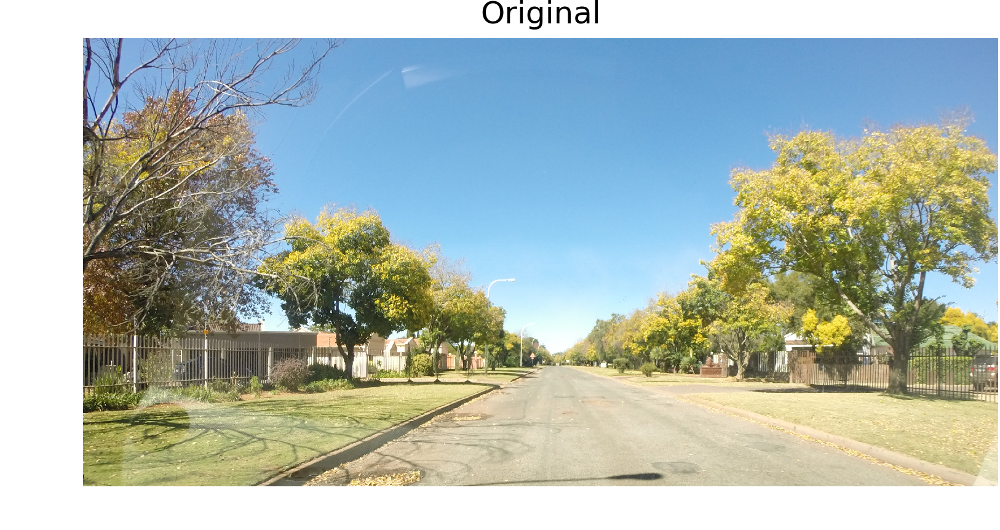
\includegraphics[scale=1]{Images/0_Original.png}
\end{center}
\caption{Pothole Image}
\end{figure}


\begin{figure}[!htb]
\begin{center}
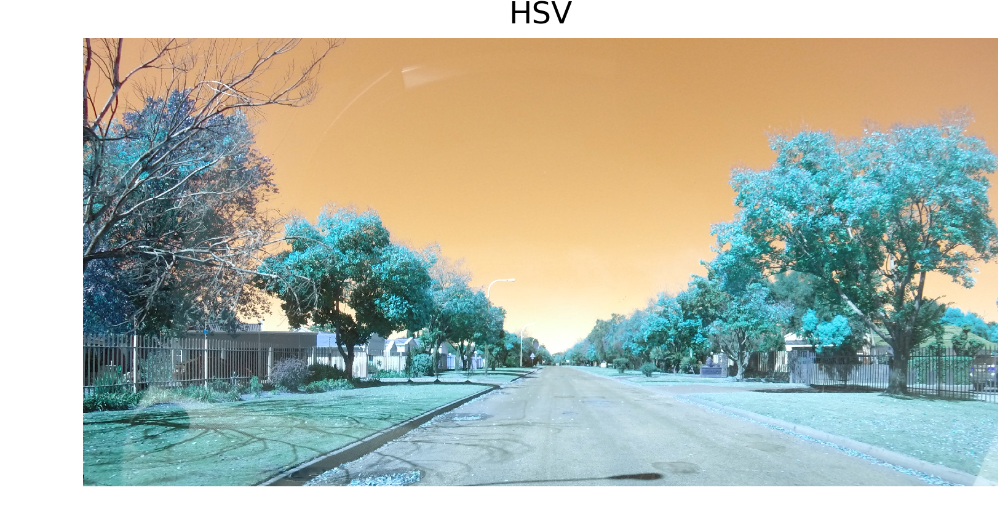
\includegraphics[scale=1]{Images/1_HSV.png}
\end{center}
\caption{Converting to HSV}
\end{figure}

\vspace{0.5cm}

\noindent From the image we selected a region of interest (ROI) where the most part of the road appears, since we are using a fixed camera mounted on the window of a moving vehicle we assume that the road area tend to appear on a fixed region above the hood of the vehicle. Hence we select a Region of Interest from the (ROI) image as show in figure 5.

\begin{figure}[!htb]
\begin{center}
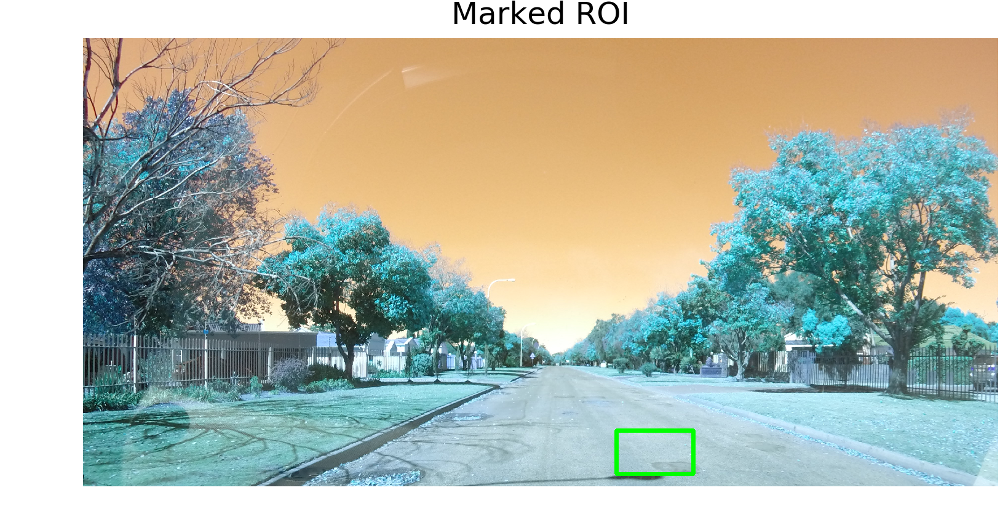
\includegraphics[scale=1]{Images/2_Marked_ROI.png}
\end{center}
\caption{Selecting the ROI}
\end{figure}

\vspace{0.5cm}

\noindent Figure 6 shows the enlarged ROI of the image. Then we convert the image to a binary image by selecting the gray scale channel. We apply thresholding on the binary image as show in the figure 7. Then the image is analysed using contour detection to find out the largest appearing contour in the selected ROI to extract the road area form the image. This largest contour servers as the mask for extracting the road. 

\begin{figure}[!htb]
\begin{center}
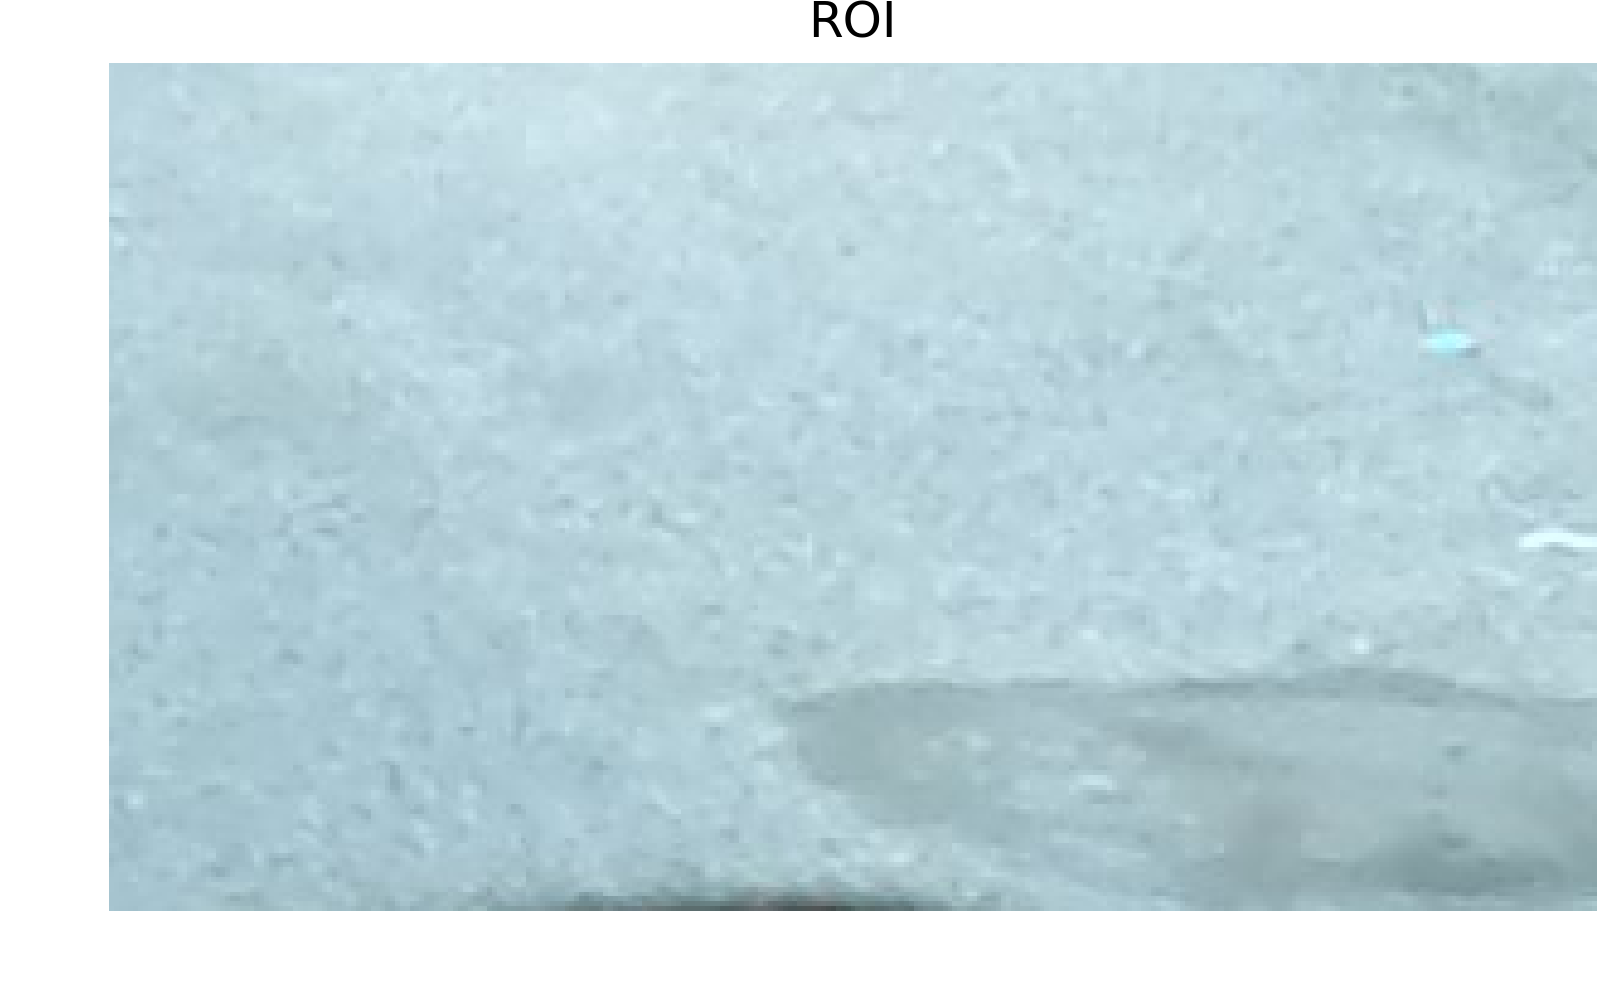
\includegraphics[scale=0.65]{Images/3_ROI.png}
\end{center}
\caption{Region of Interest}
\end{figure}

\begin{figure}[!htb]
\begin{center}
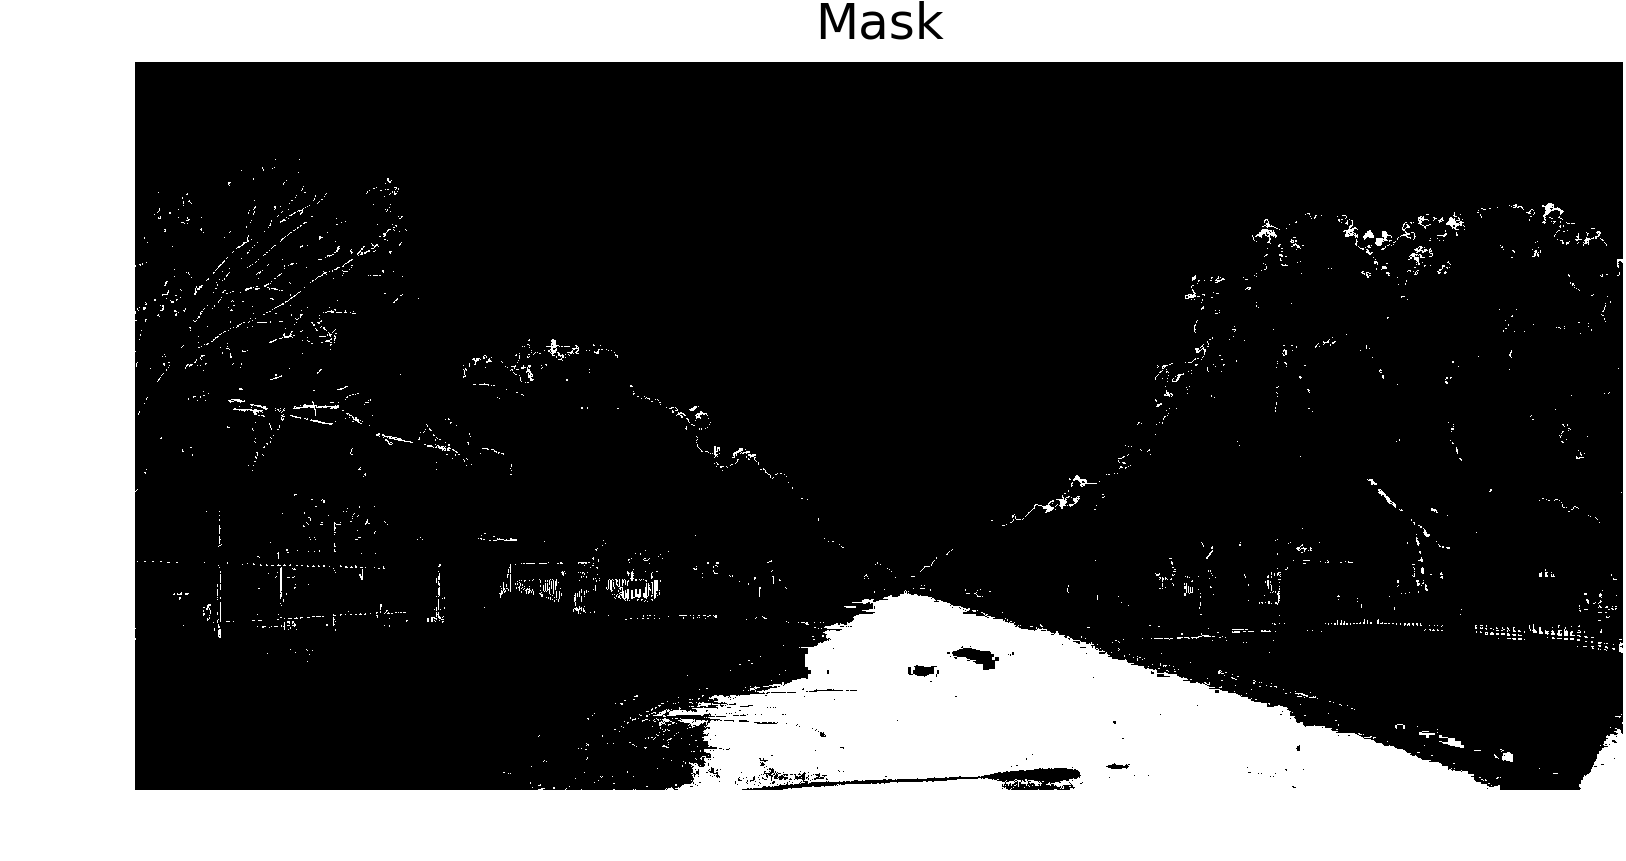
\includegraphics[scale=0.65]{Images/4_Mask.png}
\end{center}
\caption{Mask}
\end{figure}

\vspace{0.5cm}

\noindent The Figure 8 below indicated the convex hull of the largest contours selected from the thresholded images. This largest contour is used a mask to extract the road area as shown in the Figure 10.


\begin{figure}[!htb]
\begin{center}
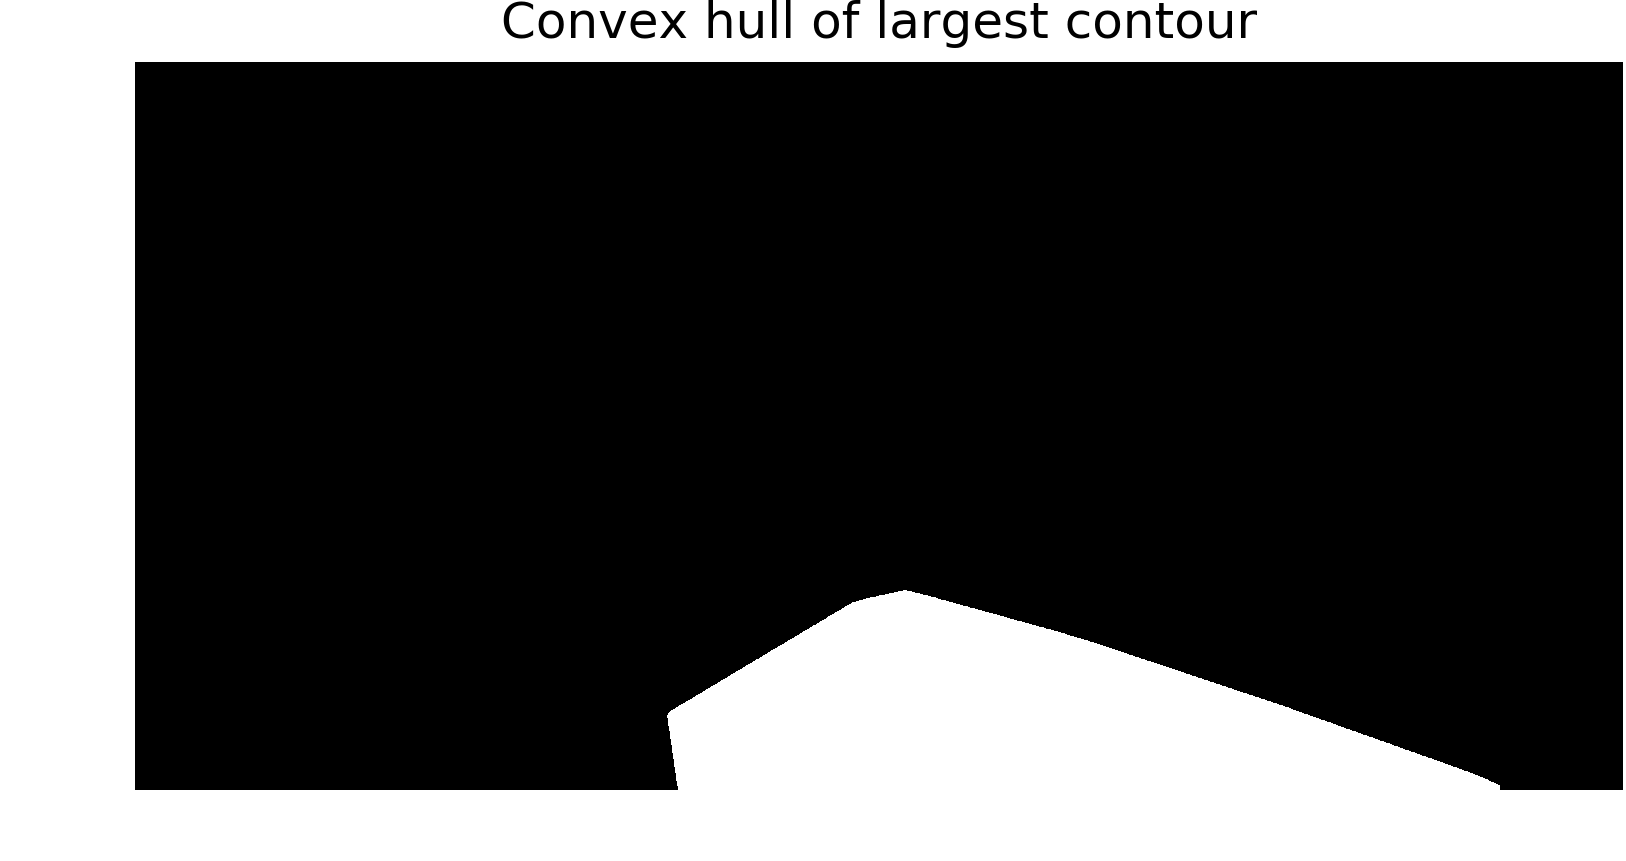
\includegraphics[scale=0.65]{Images/5_Convex_hull_of_largest_contour.png}
\end{center}
\caption{Convex hull of largest contour}
\end{figure}



\begin{figure}[!htb]
\begin{center}
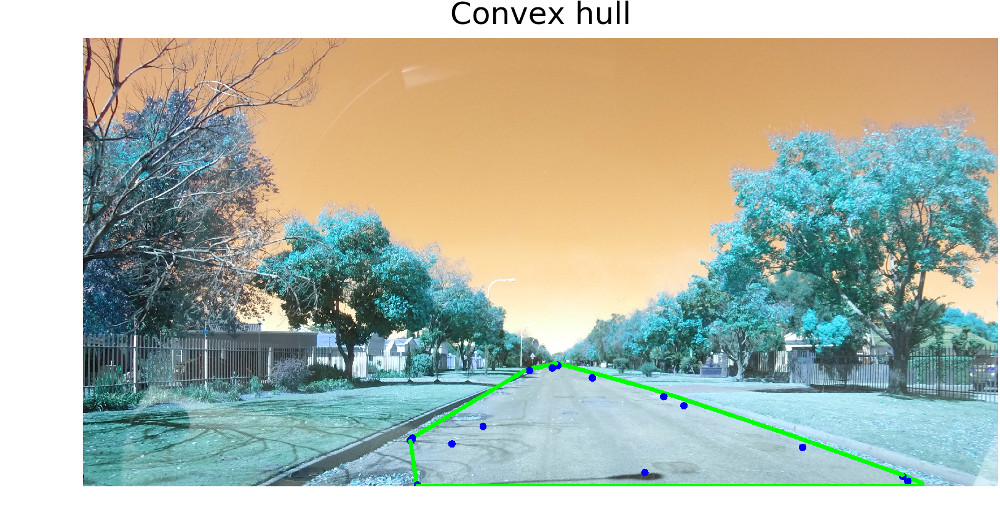
\includegraphics[scale=1]{Images/6_Convex_hull.png}
\end{center}
\caption{Convex hull on Original Image}
\end{figure}
\newpage

\begin{figure}[!htb]
\begin{center}
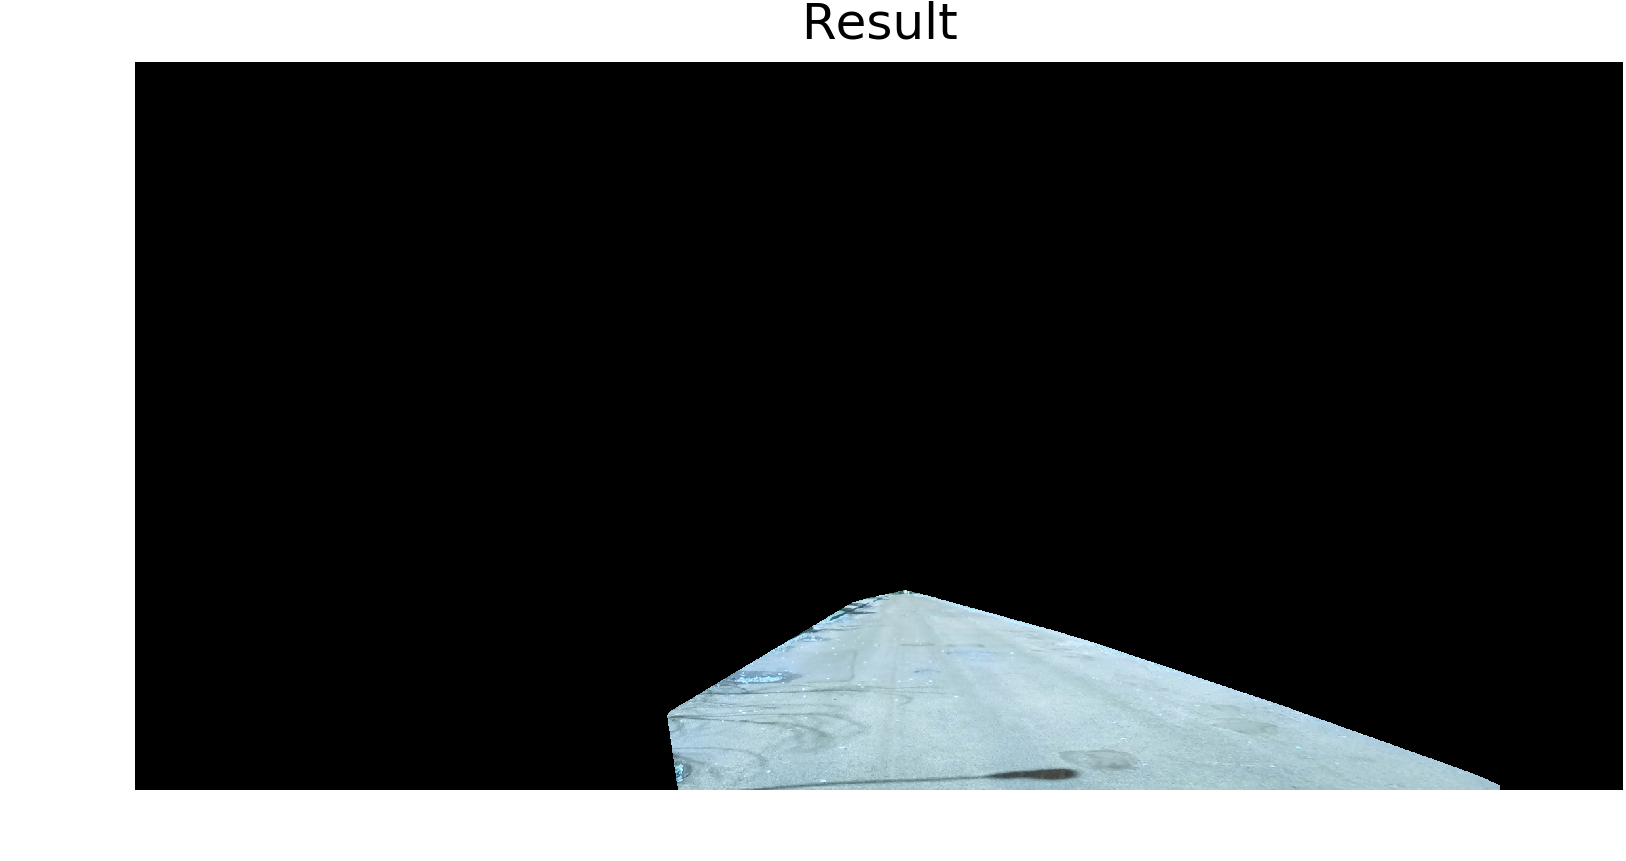
\includegraphics[scale=0.65]{Images/7_Result.png}
\end{center}
\caption{Extracted Road}
\end{figure}

\newpage

\vspace*{.5cm}


\subsubsection*{Blob Detection Method}

The extracted road area is then analysed further for pothole visualisation. In computer vision, blob detection methods are aimed at detecting regions in a digital image that differ in properties, such as brightness or color, compared to surrounding regions. Since we assume that pothole appear in the road in different texture than that of the road area mainly in dark shadowed regions some time it appear as though it is covered in mud and water. Since there is a differentiating factor that make pothole identifiable in the road we used blob detection algorithms to highlight the potholes.

\vspace*{.5cm}

\subsubsection*{Contour dilation Method}
The extracted road area could also be analysed using contour detection or edge detection (Canny edge detection) further for highlighting the presence of the potholes. But the results obtained for the potholes were sub\-optimal. Since potholes appear in varied shape and color better discrimination from other object on the road could not be achieved. 

\subsection{Pothole detection using machine learning techniques}

In this section we describe in details the various machine learning techniques that we used for detecting the presence of the pothole in the roads.

\subsubsection{Feature Modelling}

The feature extraction is done in two ways 
\begin{itemize}
\item Downscaled images as features \\
The image is downscaled(100x100) into lower resolution and then flattened to be used as a feature.
\item Color histogram as a feature \\
The color histogram of the frame is take and is used as feature for training the classifier.
\end{itemize}


\subsubsection{Machine Learning Algorithms}

The following list of machine learning techniques were used in the study. They were trained using the above mentioned feature and the results were analysed.

\begin{itemize}
\item Logistic Regression \cite{lr}
\item Decision Tree \cite{dt}
\item AdaBoost using Decision Tree
\item GaussianNB
\item KNN \cite{knn}
\item SVM \cite{svm}
\item Random Forest \cite{rf}
\end{itemize}

\section{Results}


\subsection{Pothole visualisation using Image processing Techniques}

The image processing techniques gave us suboptimal results. Method I using morphological transformation didn't work well as there are edges in the roads that created extra contours which were wrongly highlighted as potholes. Method II using road isolation followed by contour detection and edge detection worked for some scenarios but did not work well for most of the cases. Hence pothole visualisation is found difficult to achieve with the current technology as we were not able to find discriminating feature for potholes from our analysis

\subsection{Pothole detection using Machine Learning Techniques}

The classifier are trained using the feature and the results obtained are shared in the below tables.
The table below show the result obtained while using the Downscaled image as features.
\begin{center}
\begin{table}[h!]
\centering
\begin{tabular}{ |c|c| } 
 \hline
 \rowcolor{gray}
 Methods & Accuracy($\%$)  \\ 
 \hline
 Logistic Regression & 72.73 \\
 \hline
 Multinomial Logistic Regression & 68.93\\
 \hline
 Decision Tree & 86.88 \\ 
 \hline
 AdaBoost using Decision Tree & 80.32  \\ 
 \hline
 GaussianNB & 44.26 \\
 \hline
 KNN & 73.77\\
 \hline
 SVM & 55.73\\
 \hline
 Random Forest & 68.18\\
 \hline
\end{tabular}
\caption{Results for Raw downscaled images pixels as features}
\label{table:1}
\end{table}
\end{center}

\vspace{0.5cm}

The table below show the result obtained while using the color histogram as features.
\begin{center}
\begin{table}[h!]
\centering
\begin{tabular}{ |c|c| } 
 \hline
 \rowcolor{gray}
 Methods & Accuracy($\%$)  \\ 
 \hline
 Logistic Regression & 77.27\\
 \hline
 Decision Tree & 77.04 \\ 
 \hline
 AdaBoost using Decision Tree & 83.60  \\ 
 \hline
 GaussianNB & 75.40 \\
 \hline
 KNN & 78.68\\
 \hline
 SVM & 55.73\\
 \hline
 Random Forest & 95.45\\
 \hline
\end{tabular}
\caption{Results for color histogram as features}
\label{table:1}
\end{table}
\end{center}

As we can infer from the tables that the classification using downscaled images worked well when decision trees and AdaBoost using decision tree are used. Meanwhile Gaussian Naive Bayes performed the worst using downscaled images.

\vspace{0.5cm}

The color histogram as a feature worked relatively better when compared to the downscaled images. We were pretty surprised to see the performance of color histogram using Random Forest which gives at accuracy of 
95$\%$. SVM didn't give good accuracy in both color histogram as well as downscaled images.

\section{Conclusion}
We presented a mix of methods, incorporating both image processing and machine learning, to detect the presence of potholes in an image. Given an image, the road was isolated and extracted with best results using contours and finding the convex hull of the largest contour. Through successive testing, it was found that using machine learning models yielded better results than conventional image processing methods as far as detection of potholes were concerned. The models were trained using features extracted from the isolated road segment. Comparison between the different methods of feature extraction and the performance of different models on these features have also been exhibited.

\section{Future Work $\&$ Improvements}
The present work yields sub\-optimal results in scenes features heavy shadows. Better discriminating features could be extracted which helps to discern potholes even in environments where the lighting is uneven and interspersed with shadows. Methods could be developed to accommodate the presence of incoming traffic and road markings.


% use section* for acknowledgment
\section*{Acknowledgment}
We would like to thank Prof. Dinesh Babu Jayagopi for guiding us throughout this venture, Prof. MJ (Thinus) Booysen, Associate Professor at the Electrical $\&$ Electronic Engineering Department at Stellenbosch University for allowing us to use pothole datasets \cite{dataset}.

\vspace{0.5cm}

\ifCLASSOPTIONcaptionsoff
  \newpage
\fi


\appendices
\section{Data and Code}
\begin{itemize}
\item Data 
\begin{itemize}
\item Data Set I - \url{https://www.youtube.com/watch?v=hmeBmdZzlLU}
\item Data Set II - \url{https://www.youtube.com/playlist?list=PLzf2LOyk6iN3nNyvu1RI0Np-i8kT1IGE0}
\item Data Set III \cite{dataset}
\end{itemize}

\item Code - \url{https://github.com/crunchbang/MP_Project/blob/master/Code/}
\item Road Extraction Video - \url{https://www.youtube.com/watch?v=4vUqzDnZsV8}
\end{itemize}

% you can choose not to have a title for an appendix
% if you want by leaving the argument blank
%\section{}
%Appendix two text goes here.


\begin{thebibliography}{1}

\bibitem{paperone} 
S. Nienaber, M.J. Booysen, R.S. Kroon
\textit{Detecting potholes using simple image processing techniques and Real-world Footage, 2015}. 
SATC, July 2015, Pretoria, South Africa
\url{http://scholar.sun.ac.za/handle/10019.1/97191}
 
\bibitem{papertwo} 
Ajit Danti, Jyoti Y. Kulkarni, and P. S. Hiremath, Member, IACSIT
\textit{An Image Processing Approach to Detect Lanes, Pot Holes and Recognize Road Signs in Indian Roads, December 2012}
\url{http://www.ijmo.org/papers/204-S3015.pdf}

\bibitem{paperthree}
S. Nienaber, R.S. Kroon, M.J. Booysen  
\textit{“A Comparison of Low-Cost Monocular Vision Techniques for Pothole Distance Estimation”}
IEEE CIVTS, December 2015, Cape Town, South Africa.
 
\bibitem{dataset}
The annotated image dataset used in the pothole detection is freely available at
\url{https://goo.gl/3QyeMs}

\bibitem{pothole}
\url{https://en.wikipedia.org/wiki/Pothole}

\bibitem{lr}
\url{https://en.wikipedia.org/wiki/Logistic_regression}

\bibitem{dt}
\url{https://en.wikipedia.org/wiki/Decision_tree}

\bibitem{knn}
\url{https://en.wikipedia.org/wiki/K-nearest_neighbors_algorithm}

\bibitem{rf}
\url{https://en.wikipedia.org/wiki/Random_forest}

\bibitem{svm}
\url{https://en.wikipedia.org/wiki/Support_vector_machine}

\bibitem{dataset1}
Dataset with negative and positive examples separated
\url{https://drive.google.com/drive/folders/0B7LHCitTUdEYZFEwNWo4V2RldjQ?usp=sharing}

\bibitem{opencv}
Open CV is used for Image processing and Machine Learning
\url{http://docs.opencv.org/}

\end{thebibliography}

\begin{IEEEbiography}[{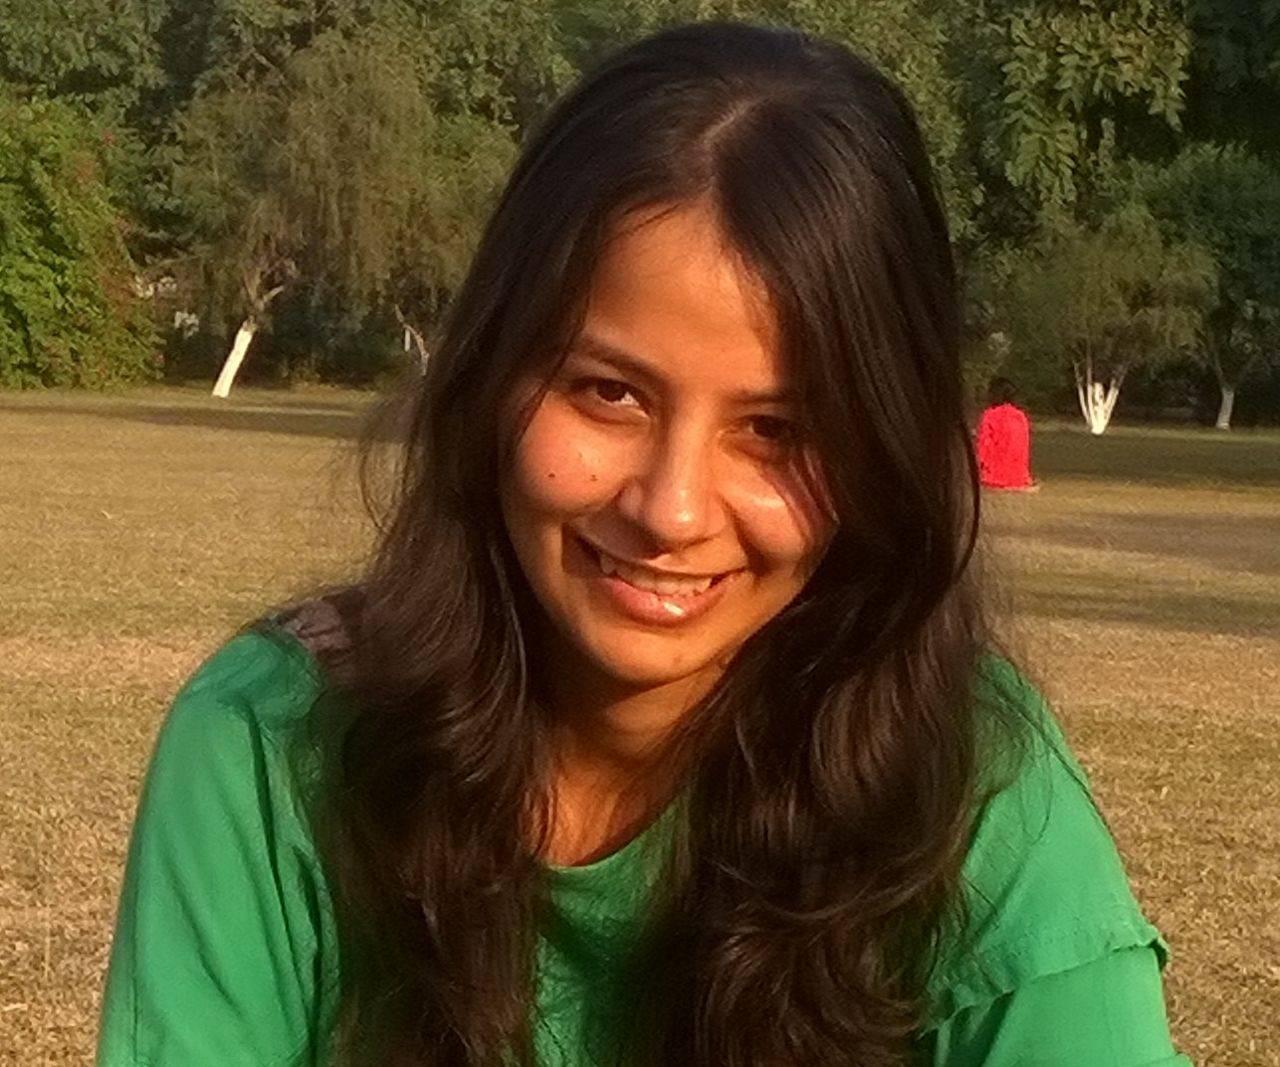
\includegraphics[width=1in,height=1.25in,clip,keepaspectratio]{Images/akanksha.jpg}}]{Akanksha Dwivedi}
(MT2016006) is currenlty pursing Master of Technology from International Institute of Information Technology, Bangalore. 
\end{IEEEbiography}

% if you will not have a photo at all:
\begin{IEEEbiography}[{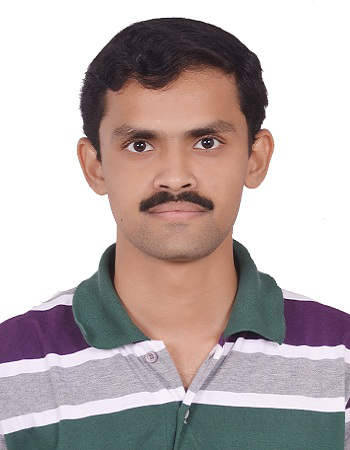
\includegraphics[width=1in,height=1.25in,clip,keepaspectratio]{anoop.jpg}}]{Anoop Toffy}
(MT2016016) is currenlty pursing Master of Technology from International Institute of Information Technology, Bangalore. 
\end{IEEEbiography}

% insert where needed to balance the two columns on the last page with
% biographies
%\newpage

\begin{IEEEbiography}[{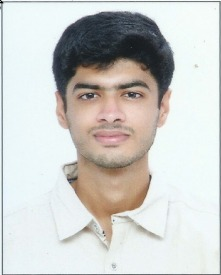
\includegraphics[width=1in,height=1.25in,clip,keepaspectratio]{Images/athul.jpg}}]{Athul Suresh}
(MT2016030) is currenlty pursing Master of Technology from International Institute of Information Technology, Bangalore. 
\end{IEEEbiography}

\begin{IEEEbiography}[{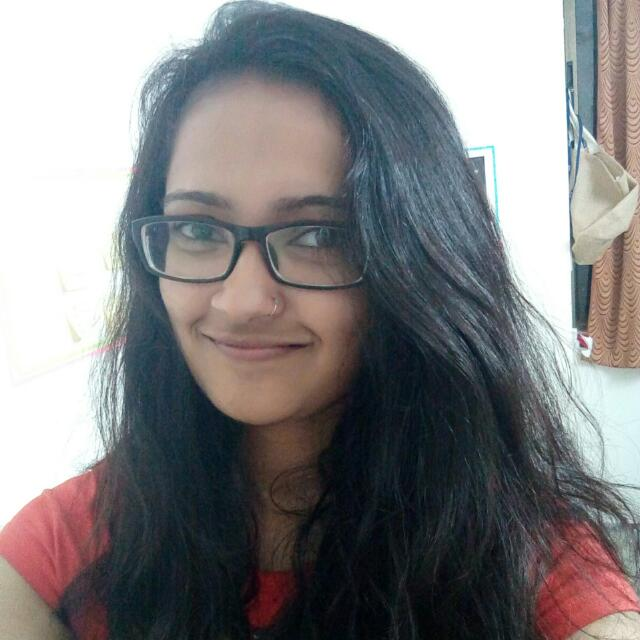
\includegraphics[width=1in,height=1.25in,clip,keepaspectratio]{Images/tarini.jpg}}]{Tarini Chandrashekhar}
(MT2016144) is currenlty pursing Master of Technology from International Institute of Information Technology, Bangalore. 

\end{IEEEbiography}

\end{document}


